\documentclass{article}
\usepackage[paperwidth=5.5in,paperheight=4.42in,margin=0pt]{geometry}
\usepackage{times,amsmath,amssymb,tikz,xcolor}
\usetikzlibrary{arrows}
\definecolor{navy}{HTML}{12464C}
\definecolor{indigo}{HTML}{357C82}
\definecolor{cyan}{HTML}{63AAA6}
\definecolor{orchid}{HTML}{C2673A}
\definecolor{mute}{HTML}{BAD0CF}
\definecolor{faint}{HTML}{DDE9E8}
\definecolor{ink}{HTML}{1F383A}
\pagestyle{empty}\setlength{\parindent}{0pt}
\begin{document}\noindent
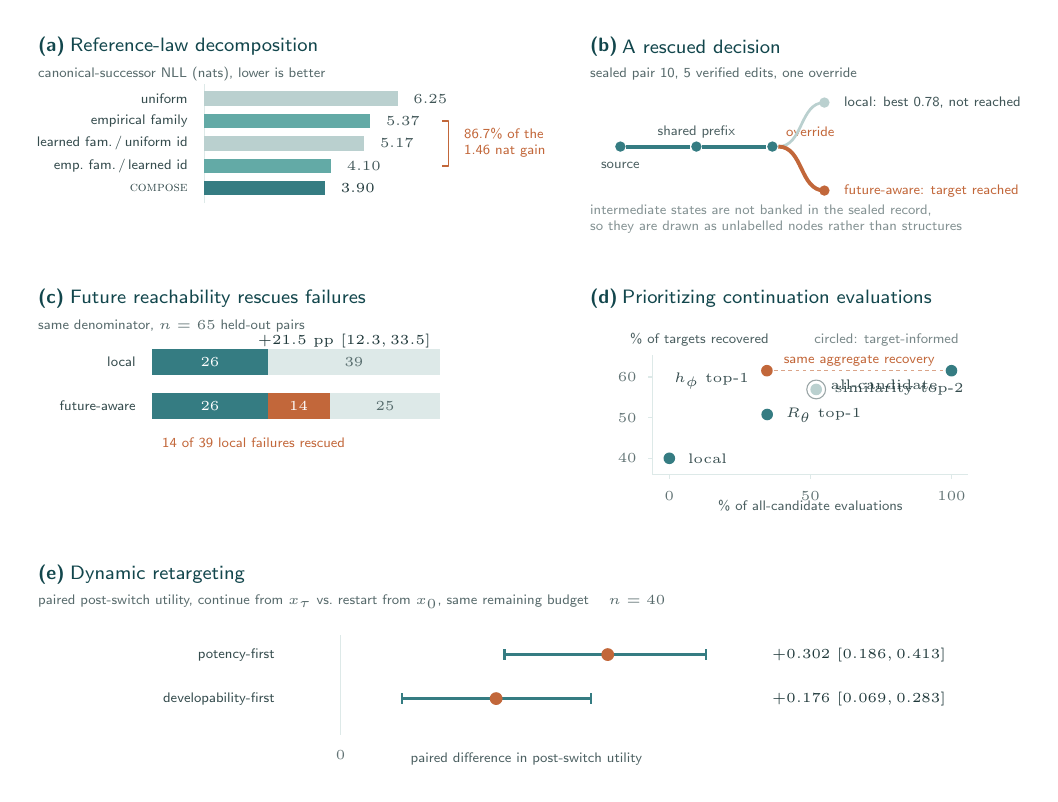
\begin{tikzpicture}[x=1in,y=1in,>=stealth,line join=round]
  \node[text=navy,anchor=west,font=\sffamily\bfseries\fontsize{7.2}{8}\selectfont] at (0.1000,4.1600) {(a)};
  \node[text=navy,anchor=west,font=\sffamily\fontsize{6.6}{7.8}\selectfont] at (0.2600,4.1600) {Reference-law decomposition};
  \node[text=ink,anchor=west,font=\sffamily\fontsize{5.5}{6.7}\selectfont,opacity=0.75] at (0.1000,4.0250) {canonical-successor NLL (nats), lower is better};
  \draw[faint,line width=0.6pt] (0.9800,3.3770) -- (0.9800,3.9750);
  \fill[mute] (0.9800,3.8640) rectangle (1.9465,3.9360);
  \node[text=ink,anchor=east,font=\sffamily\fontsize{5.0}{6.2}\selectfont,opacity=0.9] at (0.9450,3.9000) {uniform};
  \node[text=ink,anchor=west,font=\fontsize{5.2}{6.4}\selectfont,opacity=0.85] at (1.9765,3.9000) {6.25};
  \fill[cyan] (0.9800,3.7520) rectangle (1.8094,3.8240);
  \node[text=ink,anchor=east,font=\sffamily\fontsize{5.0}{6.2}\selectfont,opacity=0.9] at (0.9450,3.7880) {empirical family};
  \node[text=ink,anchor=west,font=\fontsize{5.2}{6.4}\selectfont,opacity=0.85] at (1.8394,3.7880) {5.37};
  \fill[mute] (0.9800,3.6400) rectangle (1.7794,3.7120);
  \node[text=ink,anchor=east,font=\sffamily\fontsize{5.0}{6.2}\selectfont,opacity=0.9] at (0.9450,3.6760) {learned fam.\,/\,uniform id};
  \node[text=ink,anchor=west,font=\fontsize{5.2}{6.4}\selectfont,opacity=0.85] at (1.8094,3.6760) {5.17};
  \fill[cyan] (0.9800,3.5280) rectangle (1.6135,3.6000);
  \node[text=ink,anchor=east,font=\sffamily\fontsize{5.0}{6.2}\selectfont,opacity=0.9] at (0.9450,3.5640) {emp.\ fam.\,/\,learned id};
  \node[text=ink,anchor=west,font=\fontsize{5.2}{6.4}\selectfont,opacity=0.85] at (1.6435,3.5640) {4.10};
  \fill[indigo] (0.9800,3.4160) rectangle (1.5835,3.4880);
  \node[text=ink,anchor=east,font=\sffamily\fontsize{5.0}{6.2}\selectfont,opacity=0.9] at (0.9450,3.4520) {\textsc{compose}};
  \node[text=ink,anchor=west,font=\fontsize{5.2}{6.4}\selectfont] at (1.6135,3.4520) {3.90};
  \draw[orchid,line width=0.6pt] (2.1700,3.7880) -- (2.2000,3.7880) -- (2.2000,3.5640) -- (2.1700,3.5640);
  \node[text=orchid,anchor=west,align=left,font=\sffamily\fontsize{5.0}{5.8}\selectfont] at (2.2300,3.6760) {\begin{tabular}{@{}l@{}}86.7\% of the\\1.46 nat gain\end{tabular}};
  \node[text=navy,anchor=west,font=\sffamily\bfseries\fontsize{7.2}{8}\selectfont] at (2.8600,4.1600) {(b)};
  \node[text=navy,anchor=west,font=\sffamily\fontsize{6.6}{7.8}\selectfont] at (3.0200,4.1600) {A rescued decision};
  \node[text=ink,anchor=west,font=\sffamily\fontsize{5.5}{6.7}\selectfont,opacity=0.75] at (2.8600,4.0250) {sealed pair 10, 5 verified edits, one override};
  \draw[indigo,line width=1.4pt] (3.0900,3.6600) -- (3.4100,3.6600);
  \draw[indigo,line width=1.4pt] (3.4700,3.6600) -- (3.7900,3.6600);
  \fill[indigo] (3.0600,3.6600) circle (0.026);
  \fill[indigo] (3.4400,3.6600) circle (0.026);
  \fill[indigo] (3.8200,3.6600) circle (0.026);
  \node[text=ink,anchor=center,font=\sffamily\fontsize{5.0}{6.2}\selectfont,opacity=0.8] at (3.0600,3.5650) {source};
  \node[text=ink,anchor=center,font=\sffamily\fontsize{5.0}{6.2}\selectfont,opacity=0.8] at (3.4400,3.7350) {shared prefix};
  \node[text=orchid,anchor=west,font=\sffamily\fontsize{5.0}{6.2}\selectfont] at (3.8400,3.7350) {override};
  \draw[mute,line width=1.0pt] (3.8500,3.6600) to[out=0,in=180] (4.0800,3.8800);
  \fill[mute] (4.0800,3.8800) circle (0.026);
  \node[text=ink,anchor=west,font=\sffamily\fontsize{5.0}{6.2}\selectfont,opacity=0.85] at (4.1300,3.8800) {local: best 0.78, not reached};
  \draw[orchid,line width=1.4pt] (3.8500,3.6600) to[out=0,in=180] (4.0800,3.4400);
  \fill[orchid] (4.0800,3.4400) circle (0.026);
  \node[text=orchid,anchor=west,font=\sffamily\fontsize{5.0}{6.2}\selectfont] at (4.1300,3.4400) {future-aware: target reached};
  \node[text=ink,anchor=west,font=\sffamily\fontsize{4.7}{5.9}\selectfont,opacity=0.55] at (2.8600,3.3400) {intermediate states are not banked in the sealed record,};
  \node[text=ink,anchor=west,font=\sffamily\fontsize{4.7}{5.9}\selectfont,opacity=0.55] at (2.8600,3.2600) {so they are drawn as unlabelled nodes rather than structures};
  \node[text=navy,anchor=west,font=\sffamily\bfseries\fontsize{7.2}{8}\selectfont] at (0.1000,2.9000) {(c)};
  \node[text=navy,anchor=west,font=\sffamily\fontsize{6.6}{7.8}\selectfont] at (0.2600,2.9000) {Future reachability rescues failures};
  \node[text=ink,anchor=west,font=\sffamily\fontsize{5.5}{6.7}\selectfont,opacity=0.75] at (0.1000,2.7650) {same denominator, $n=65$ held-out pairs};
  \node[text=ink,anchor=east,font=\sffamily\fontsize{5.2}{6.4}\selectfont,opacity=0.9] at (0.6850,2.5840) {local};
  \fill[indigo] (0.7200,2.5200) rectangle (1.2960,2.6480);
  \node[text=white,anchor=center,font=\fontsize{5.0}{6.2}\selectfont] at (1.0080,2.5840) {26};
  \fill[faint] (1.2960,2.5200) rectangle (2.1600,2.6480);
  \node[text=ink,anchor=center,font=\fontsize{5.0}{6.2}\selectfont,opacity=0.7] at (1.7280,2.5840) {39};
  \node[text=ink,anchor=east,font=\sffamily\fontsize{5.2}{6.4}\selectfont,opacity=0.9] at (0.6850,2.3640) {future-aware};
  \fill[indigo] (0.7200,2.3000) rectangle (1.2960,2.4280);
  \node[text=white,anchor=center,font=\fontsize{5.0}{6.2}\selectfont] at (1.0080,2.3640) {26};
  \fill[orchid] (1.2960,2.3000) rectangle (1.6062,2.4280);
  \node[text=white,anchor=center,font=\fontsize{5.0}{6.2}\selectfont] at (1.4511,2.3640) {14};
  \fill[faint] (1.6062,2.3000) rectangle (2.1600,2.4280);
  \node[text=ink,anchor=center,font=\fontsize{5.0}{6.2}\selectfont,opacity=0.7] at (1.8831,2.3640) {25};
  \node[text=orchid,anchor=west,font=\sffamily\fontsize{5.0}{6.2}\selectfont] at (0.7200,2.1800) {14 of 39 local failures rescued};
  \node[text=ink,anchor=east,font=\fontsize{5.4}{6.6000000000000005}\selectfont] at (2.1600,2.6900) {$+21.5$ pp $[12.3, 33.5]$};
  \node[text=navy,anchor=west,font=\sffamily\bfseries\fontsize{7.2}{8}\selectfont] at (2.8600,2.9000) {(d)};
  \node[text=navy,anchor=west,font=\sffamily\fontsize{6.6}{7.8}\selectfont] at (3.0200,2.9000) {Prioritizing continuation evaluations};
  \node[text=ink,anchor=west,font=\sffamily\fontsize{5.5}{6.7}\selectfont,opacity=0.75] at (2.8600,2.7650) {};
  \draw[faint,line width=0.6pt] (3.2200,2.0200) -- (3.2200,2.6200);
  \draw[faint,line width=0.6pt] (3.2200,2.0200) -- (4.8000,2.0200);
  \draw[faint,line width=0.5pt] (3.3046,2.0000) -- (3.3046,2.0200);
  \node[text=ink,anchor=north,font=\fontsize{4.8}{6.0}\selectfont,opacity=0.7] at (3.3046,1.9840) {0};
  \draw[faint,line width=0.5pt] (4.0100,2.0000) -- (4.0100,2.0200);
  \node[text=ink,anchor=north,font=\fontsize{4.8}{6.0}\selectfont,opacity=0.7] at (4.0100,1.9840) {50};
  \draw[faint,line width=0.5pt] (4.7154,2.0000) -- (4.7154,2.0200);
  \node[text=ink,anchor=north,font=\fontsize{4.8}{6.0}\selectfont,opacity=0.7] at (4.7154,1.9840) {100};
  \draw[faint,line width=0.5pt] (3.2000,2.1014) -- (3.2200,2.1014);
  \node[text=ink,anchor=east,font=\fontsize{4.8}{6.0}\selectfont,opacity=0.7] at (3.1900,2.1014) {40};
  \draw[faint,line width=0.5pt] (3.2000,2.3047) -- (3.2200,2.3047);
  \node[text=ink,anchor=east,font=\fontsize{4.8}{6.0}\selectfont,opacity=0.7] at (3.1900,2.3047) {50};
  \draw[faint,line width=0.5pt] (3.2000,2.5081) -- (3.2200,2.5081);
  \node[text=ink,anchor=east,font=\fontsize{4.8}{6.0}\selectfont,opacity=0.7] at (3.1900,2.5081) {60};
  \node[text=ink,anchor=center,font=\sffamily\fontsize{4.8}{6.0}\selectfont,opacity=0.8] at (4.0100,1.8650) {\% of all-candidate evaluations};
  \node[text=ink,anchor=west,font=\sffamily\fontsize{4.8}{6.0}\selectfont,opacity=0.8] at (3.0600,2.6950) {\% of targets recovered};
  \draw[orchid,line width=0.5pt,dash pattern=on 1.3pt off 1.3pt,opacity=0.6] (3.7925,2.5394) -- (4.7154,2.5394);
  \node[text=orchid,anchor=center,font=\sffamily\fontsize{4.6}{5.8}\selectfont] at (4.2539,2.5874) {same aggregate recovery};
  \fill[indigo] (3.3046,2.1014) circle (0.029);
  \node[text=ink,anchor=west,font=\fontsize{4.8}{6.0}\selectfont,opacity=0.9] at (3.3496,2.1014) {local};
  \fill[indigo] (3.7938,2.3204) circle (0.029);
  \node[text=ink,anchor=west,font=\fontsize{4.8}{6.0}\selectfont,opacity=0.9] at (3.8388,2.3154) {$R_\theta$ top-1};
  \fill[orchid] (3.7925,2.5394) circle (0.029);
  \node[text=ink,anchor=east,font=\fontsize{4.8}{6.0}\selectfont,opacity=0.9] at (3.7505,2.4874) {$h_\phi$ top-1};
  \fill[mute] (4.0389,2.4456) circle (0.029);
  \draw[ink,opacity=0.45,line width=0.4pt] (4.0389,2.4456) circle (0.047);
  \node[text=ink,anchor=west,font=\fontsize{4.8}{6.0}\selectfont,opacity=0.9] at (4.0839,2.4456) {similarity top-2};
  \fill[indigo] (4.7154,2.5394) circle (0.029);
  \node[text=ink,anchor=east,font=\fontsize{4.8}{6.0}\selectfont,opacity=0.9] at (4.6954,2.4674) {all-candidate};
  \node[text=ink,anchor=east,font=\sffamily\fontsize{4.6}{5.8}\selectfont,opacity=0.6] at (4.8000,2.6950) {circled: target-informed};
  \node[text=navy,anchor=west,font=\sffamily\bfseries\fontsize{7.2}{8}\selectfont] at (0.1000,1.5200) {(e)};
  \node[text=navy,anchor=west,font=\sffamily\fontsize{6.6}{7.8}\selectfont] at (0.2600,1.5200) {Dynamic retargeting};
  \node[text=ink,anchor=west,font=\sffamily\fontsize{5.5}{6.7}\selectfont,opacity=0.75] at (0.1000,1.3850) {paired post-switch utility, continue from $x_\tau$ vs.\ restart from $x_0$, same remaining budget \quad $n=40$};
  \draw[faint,line width=0.6pt] (1.6612,0.7200) -- (1.6612,1.2200);
  \node[text=ink,anchor=north,font=\fontsize{4.8}{6.0}\selectfont,opacity=0.7] at (1.6612,0.6900) {0};
  \node[text=ink,anchor=east,font=\sffamily\fontsize{5.2}{6.4}\selectfont,opacity=0.9] at (1.3800,1.1200) {potency-first};
  \draw[indigo,line width=1.0pt] (2.4816,1.1200) -- (3.4880,1.1200);
  \draw[indigo,line width=1.0pt] (2.4816,1.0940) -- (2.4816,1.1460);
  \draw[indigo,line width=1.0pt] (3.4880,1.0940) -- (3.4880,1.1460);
  \fill[orchid] (2.9967,1.1200) circle (0.032);
  \node[text=ink,anchor=west,font=\fontsize{5.2}{6.4}\selectfont] at (3.7700,1.1200) {$+0.302$ $[0.186, 0.413]$};
  \node[text=ink,anchor=east,font=\sffamily\fontsize{5.2}{6.4}\selectfont,opacity=0.9] at (1.3800,0.9000) {developability-first};
  \draw[indigo,line width=1.0pt] (1.9679,0.9000) -- (2.9133,0.9000);
  \draw[indigo,line width=1.0pt] (1.9679,0.8740) -- (1.9679,0.9260);
  \draw[indigo,line width=1.0pt] (2.9133,0.8740) -- (2.9133,0.9260);
  \fill[orchid] (2.4387,0.9000) circle (0.032);
  \node[text=ink,anchor=west,font=\fontsize{5.2}{6.4}\selectfont] at (3.7700,0.9000) {$+0.176$ $[0.069, 0.283]$};
  \node[text=ink,anchor=center,font=\sffamily\fontsize{4.8}{6.0}\selectfont,opacity=0.8] at (2.5900,0.6000) {paired difference in post-switch utility};
\end{tikzpicture}
\end{document}
